\documentclass[a4paper,11pt]{book}
\usepackage{listings}
\usepackage{dirtree}
\usepackage[utf8]{inputenc}
\usepackage{titlesec}
\usepackage{fancyhdr}
\usepackage[spanish,es-tabla]{babel}
\usepackage[hidelinks]{hyperref}
\usepackage{xcolor}
\usepackage{pdfpages}
\usepackage{url}
\usepackage{booktabs}
\usepackage[export]{adjustbox}
\usepackage{fancybox}
\usepackage{caption}

\usepackage{textcomp}

\usepackage{wrapfig}


\usepackage{float}

\usepackage{booktabs}

\usepackage{rotating}

% Información reutilizable
\newcommand{\asunto}{Inteligencia Computacional}
\newcommand{\titulo}{Resolución de Problemas de Asignación Cuadrática con Algoritmos Evolutivos}
\newcommand{\grado}{Máster en Ingeniería Informática}
\newcommand{\autor}{Pedro Manuel Gómez-Portillo López}
\newcommand{\email}{gomezportillo@correo.ugr.es}
\newcommand{\profesor}{Fernando Berzal Galiano}
\newcommand{\escuela}{Escuela Técnica Superior de Ingenierías Informática y de Telecomunicación}
\newcommand{\universidad}{Universidad de Granada}
\newcommand{\ciudad}{Granada}
\newcommand{\vers}{Versión 1.0}
\providecommand{\keywords}{algoritmos evolutivos, problemas de asignación cuadrática, qap}

\providecommand{\keywordsen}{evolutionary algorithm, quadratic assignment problem, qap}


% Información archivo
\hypersetup{
pdfauthor = {\autor\ (\email)},
pdftitle = {\titulo},
pdfsubject = {\asunto},
pdfkeywords = {\keywords},
pdfcreator = {MacTeX con el paquete TeX Live},
pdfproducer = {pdflatex}
}

% Estilo de cabeceras
\pagestyle{fancy}
\fancyhf{}
\fancyhead[LO]{\leftmark}
\fancyhead[RE]{\rightmark}
\fancyhead[RO,LE]{\textbf{\thepage}}
\setlength{\headheight}{1.5\headheight}

\setlength{\parskip}{0.5em}

% Redefinición de comandos
\renewcommand{\lstlistingname}{Fragmento de código}
\renewcommand{\lstlistlistingname}{Índice de fragmentos de código}
\renewcommand{\chaptermark}[1]{\markboth{\textbf{#1}}{}}
\renewcommand{\sectionmark}[1]{\markright{\textbf{\thesection. #1}}}

% Definición de colores
\definecolor{gray97}{gray}{.97}
\definecolor{gray75}{gray}{.75}
\definecolor{gray45}{gray}{.45}
\definecolor{gray30}{gray}{.94}
\definecolor{lightgray}{rgb}{.9,.9,.9}
\definecolor{darkgray}{rgb}{.4,.4,.4}
\definecolor{purple}{rgb}{0.65, 0.12, 0.82}
\definecolor{background}{HTML}{EEEEEE}
\definecolor{delim}{RGB}{20,105,176}
\colorlet{punct}{red!60!black}
\colorlet{numb}{magenta!60!black}

\definecolor{dkgreen}{rgb}{0,0.6,0}
\definecolor{gray}{rgb}{0.5,0.5,0.5}
\definecolor{mauve}{rgb}{0.58,0,0.82}

% Listados
\lstset{
aboveskip=0.5cm,
backgroundcolor=\color{gray97},
basicstyle=\scriptsize\ttfamily,
breaklines=true,
%commentstyle=\color{gray45},
frame=Ltb,
framerule=0.5pt,
framesep=0pt,
framexbottommargin=3pt,
framexleftmargin=0.1cm,
framextopmargin=3pt,
%keywordstyle=\bfseries,
numberfirstline = false,
numbers=left,
numbersep=6pt,
%numberstyle=\tiny,
rulesep=.4pt,
rulesepcolor=\color{black},
showstringspaces = false,
%stringstyle=\ttfamily,
numberstyle=\tiny\color{gray},
keywordstyle=\color{blue},
commentstyle=\color{dkgreen},
stringstyle=\color{mauve},
literate={á}{{\'a}}1
{é}{{\'e}}1
{í}{{\'i}}1
{ó}{{\'o}}1
{ú}{{\'u}}1
{ñ}{{\~n}}1
}


% Minimizar fragmentado de listados
\lstnewenvironment{listing}[1][]
{\lstset{#1}\pagebreak[0]}{\pagebreak[0]}

% Listado definido para JavaScript
% http://tex.stackexchange.com/questions/89574/language-option-supported-in-listings/89576#89576
\lstdefinelanguage{javascript}{
backgroundcolor=\color{background},
basicstyle=\footnotesize,
breaklines=true,
captionpos=b,
comment=[l]{//},
commentstyle=\color{purple}\ttfamily,
frame=lines,
identifierstyle=\color{black},
keywordstyle=\color{blue}\bfseries,
morecomment=[s]{/*}{*/},
morestring=[b]',
morestring=[b]",
ndkeywordstyle=\color{darkgray}\bfseries,
numbers=left,
numbersep=8pt,
numberstyle=\scriptsize,
sensitive=false,
showstringspaces=false,
stepnumber=1,
stringstyle=\color{red}\ttfamily,
keywords={
break,
case,
catch,
catch,
do,
else,
false,
function,
if,
in,
new,
null,
return,
switch,
true,
typeof,
var,
while},
ndkeywords={
boolean,
class,
export,
implements,
import,
this,
throw}
}

% Listado definido para JSON
% http://tex.stackexchange.com/questions/83085/how-to-improve-listings-display-of-json-files/83100#83100
\lstdefinelanguage{json}{
backgroundcolor=\color{background},
basicstyle=\footnotesize,
breaklines=true,
captionpos=b,
frame=lines,
numbers=left,
numbersep=8pt,
numberstyle=\scriptsize,
showstringspaces=false,
stepnumber=1,
literate=
*{:}{{{\color{punct}{:}}}}{1}
{,}{{{\color{punct}{,}}}}{1}
{\{}{{{\color{delim}{\{}}}}{1}
{\}}{{{\color{delim}{\}}}}}{1}
{[}{{{\color{delim}{[}}}}{1}
{]}{{{\color{delim}{]}}}}{1}
{ñ}{{\~{n}}}{1}
}

% Para que las páginas en blanco no tengan cabecera
\makeatletter
\def\clearpage{%
\ifvmode
\ifnum \@dbltopnum =\m@ne
\ifdim \pagetotal <\topskip
\hbox{}
\fi
\fi
\fi
\newpage
\thispagestyle{empty}
\write\m@ne{}
\vbox{}
\penalty -\@Mi
}
\makeatother

\begin{document}
\begin{titlepage}

  \newlength{\centeroffset}
  \setlength{\centeroffset}{-0.5\oddsidemargin}
  \addtolength{\centeroffset}{0.5\evensidemargin}

  \noindent\hspace*{\centeroffset}\begin{minipage}{\textwidth}

  \centering
  
\includegraphics[width=0.9\textwidth]{../images/logo_ugr.png}\\[1.4cm]

  \textsc{\Large\asunto\\[0.2cm]}
  \textsc{\grado}\\[1cm]

  {\Huge\bfseries \titulo\\}
  \noindent\rule[-1ex]{\textwidth}{3pt}\\[3.5ex]

  \vspace*{1.25cm}

  \centering

  \textbf{Autor}\\

  \vspace*{0.25cm}

  {\autor} \\

  \vspace*{0.25cm}

  \url{\email} \\
  % \textbf{Profesor}\\ {\profesor}\\[2cm]
  % 
\includegraphics[width=0.3\textwidth]{../images/logo_etsiit.png}\\[0.1cm]

  \vspace*{2.25cm}

  \textsc{\escuela}\\
  \textsc{---}\\
  \ciudad, \today\\
  % \includegraphics[width=0.3\textwidth]{../images/CC-SA-logo.png}
\end{minipage}
\end{titlepage}

\frontmatter
\newpage
\thispagestyle{empty}

\begin{center}

\vspace*{\fill}

El formato de la documentación de este trabajo ha sido basado en la plantilla \LaTeX\space de \href{https://github.com/erseco}{https://github.com/erseco}.

\end{center}

\newpage

\begin{center}
  {\LARGE\bfseries\titulo}\\
\end{center}
\begin{center}
  \autor\
\end{center}

\section*{Resumen}

\bigskip

Los algoritmos evolutivos son métodos de optimización y búsqueda de soluciones basados en la Teoría de la Evolución de las especies.

\bigskip

En esta práctica se trabajará con algoritmos evolutivos para resolver un problema de asignación cuadrática. Para ello, tras diseñar e implementar un algoritmo evolutivo estándar, se diseñarán sus variantes lamarckiana y baldwiniana y se compararán los resultados obtenidos tras su ejecución con el fin de descubrir cuál se desempeña mejor en este problema en concreto.

\bigskip

% \noindent{\textbf{Palabras clave}: \textit{\keywords}\\
\subsection*{Palabras clave}
\textit{\keywords}\\

\subsection*{Keywords}
\textit{\keywordsen}\\

\begingroup
\let\cleardoublepage\clearpage
\tableofcontents
\endgroup
\thispagestyle{empty}

\begingroup
\let\cleardoublepage\clearpage
\listoffigures
\endgroup
\thispagestyle{empty}

% \begingroup
% \let\cleardoublepage\clearpage
% \listoftables
% \endgroup
% \thispagestyle{empty}
\
\mainmatter
\chapter{Introducción}

Los algoritmos evolutivos son métodos de optimización y búsqueda de soluciones basados en la Teoría de la Evolución de las especies. Según ésta, un conjunto de individuos forma una generación y éstos, al reproducirse entre ellos, generan nuevos individuos con características comunes de ambos padres.

Actualmente existe una gran cantidad de aplicaciones que hacen uso de los algoritmos evolutivos para toda clase de tareas; desde estrategias de búsqueda a problemas de optimización.


Un subtipo de los problemas de optimización son los problemas de optimización cuadrática, o \textit{QAP}\footnote{Quadratic Asignation Problem} por sus siglas en inglés,  que son problemas de optimización combinatoria. Dicho problema puede describirse de la siguiente forma.


Supongamos que queremos decidir dónde construir \texttt{n} instalaciones (p.ej. fábricas) y tenemos \texttt{n} posibles localizaciones en las que podemos construir dichas instalaciones. Conocemos las distancias que hay entre cada par de instalaciones y también el flujo de materiales que ha de existir entre ellas. El problema consiste en decidir dónde ubicar cada fábrica para minimizar el coste de transporte de materiales.


Formalmente, si llamamos \texttt{d(i, j)} a la distancia de la localización \texttt{i} a la localización \texttt{j} y \texttt{w(i, j)} al peso asociado al flujo de materiales que ha de transportarse de la instalación \texttt{i} a la instalación \texttt{j}, hemos de encontrar la asignación de instalaciones a localizaciones que minimice la función de coste

\[ \sum_{i,j} w(i,j) d(p(i),p(j)) \]
\label{formula:sum}

donde \texttt{p()} define una permutación sobre el conjunto de instalaciones.

El ejemplo clásico de este tipo de problemas es el \textit{TSP}\footnote{Travel Salesman Problem} o Problema del Viajante, donde el objetivo es encontrar la ruta más corta entre varias ciudades.


\begin{figure}[H]
  \centering
  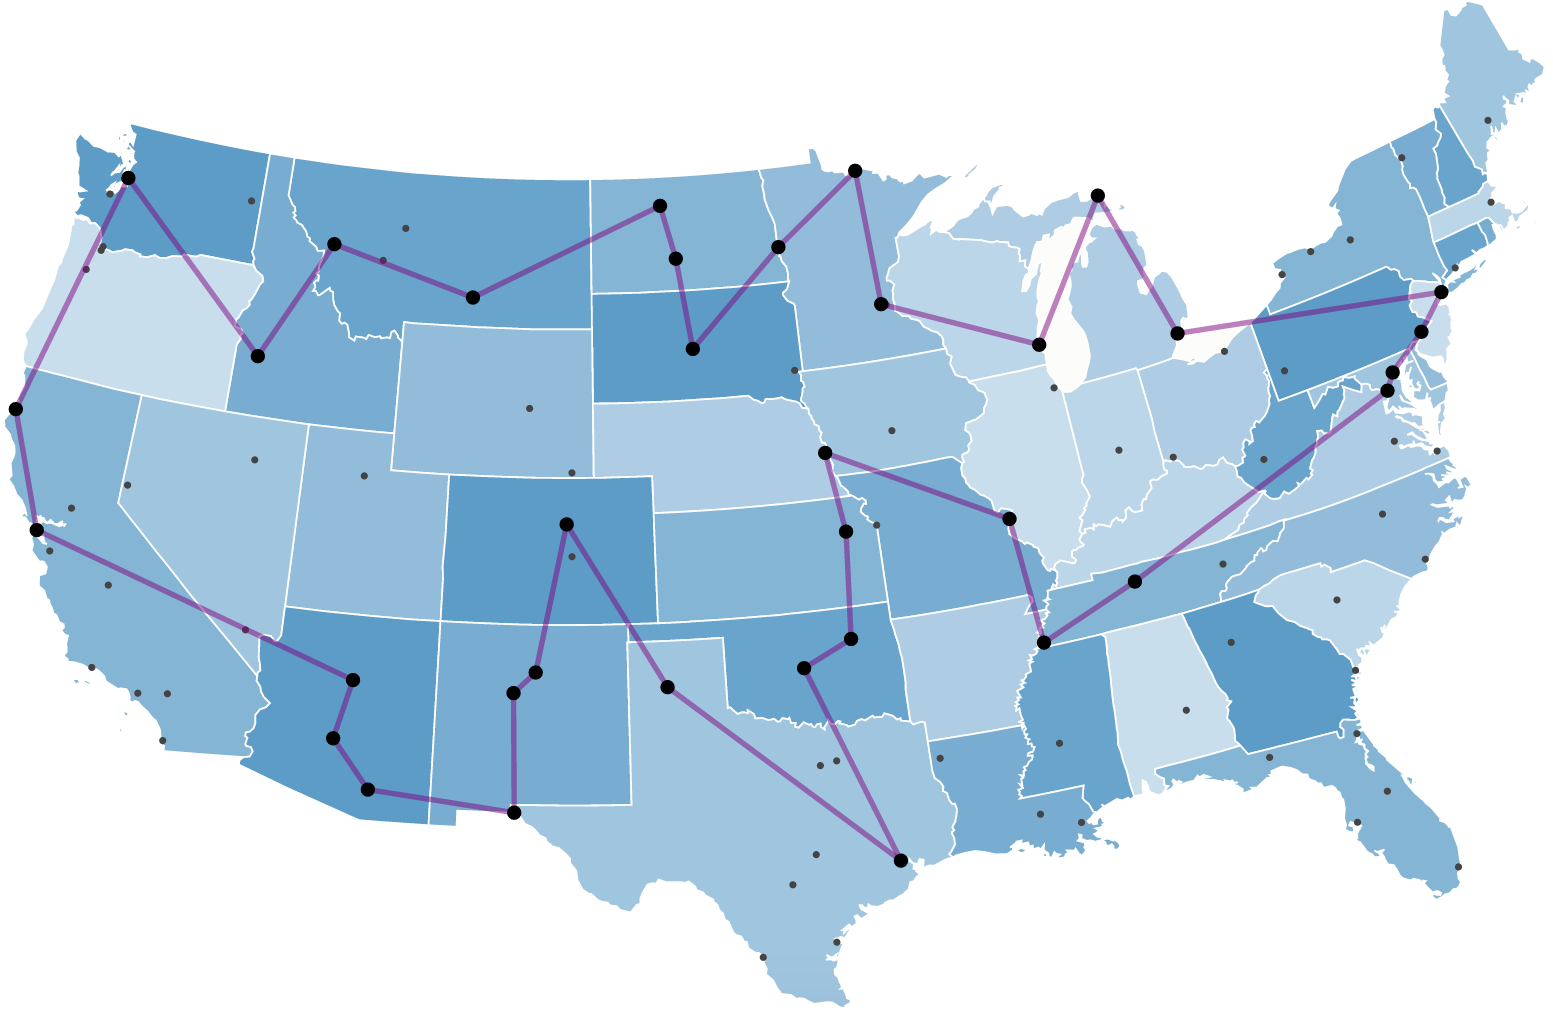
\includegraphics[width=0.65\textwidth]{../images/tsp}
  \caption{Ejemplo de rutas entre ciudades}
  \label{fig:tsp}
\end{figure}


Los casos de prueba para comprobar el funcionamiento de las distintas heurísticas se han obtenido de la biblioteca \textit{QAPLIB}\footnote{\url{(http://www.seas.upenn.edu/qaplib/}}. Cada uno de los archivos contiene el tamaño del problema, la matriz de flujo y la matriz de distancias.

En esta práctica sólo se trabajará con el archivo \texttt{tai256c}, cuyo tamaño es de 256. A día de hoy, la cota inferior global conocida (la mejor solución que se ha obtenido) tiene un fitness de 44,095,032, por lo que se supondrá que cualquier resultado que se obtenga menor a este será erróneo.


\section{Entorno de desarrollo}

Mi ordenador personal, en el cual se ha realizado esta práctica, cuenta con las siguientes características.

\begin{itemize}
  \item \textbf{Sistema operativo}. Windows 10 Educational
  \item \textbf{Procesador}. Intel Core i7-6700HQ Quad-Core 2.6GHz
  \item \textbf{Cache}. 6M
  \item \textbf{Memoria RAM}. 8GB DDR4 2,133MHz
  \item \textbf{Tarjeta gráfica}. NVIDIA 950M 
  \item \textbf{Disco duro}. SanDisk SSD Plus 256GB
  \item \textbf{Lenguaje de programación}. Python 3.7
\end{itemize}

\section{Repositorio}

El desarrollo y la evolución de esta práctica pueden verse en el siguiente repositorio.

\begin{center}
\url{https://github.com/gomezportillo/qap}
\end{center}
% \input{chapters/02_EstadoArte}
\chapter{Implementación}
\label{chap:impl}

La figura \ref{fig:class-diagram} presenta el diagrama de clases del proyecto, que ha sido creada con la herramienta de generación automática de clases a partir de código de \textit{Visual Paradigm}\footnote{\url{https://www.visual-paradigm.com/}}.

Se ha diseñado la clase \texttt{Genetic\_Algorithm}, de la que heredan el resto de algoritmos, que contiene las variables y métodos comunes; esta clase define el tamaño y el número de las generaciones, parsea el fichero de datos, crea las generaciones\dots

De ella heredan tres clases; la implementación estándar del problema, \texttt{Standard}, la variante lamarckiana, \texttt{Lamarckian}, y la variante Baldwiniana, \texttt{Baldwinian}.

La clase \texttt{Individual}, que usan el resto de clases, representa a los individuos del algoritmo; estos individuos tienen un array que representa sus \textbf{cromosomas} (generados aleatoriamente) y otras herramientas, como funciones que permiten mutarlos conforme a una probabilidad, y un \textbf{fitness}, que indica cómo de óptimos son sus cromosomas.

Como \textbf{mecanismo de selección} se ha utilizado un \textbf{torneo binario}. En él, se eligen dos individuos al azar de la población actual y se devuelve aquél con menor fitness.

Como \textbf{mecanismo de reemplazo} se utiliza el \textbf{elitismo}; el mejor individuo de una generación pasa automáticamente a la siguiente, sustituyendo al peor de ésta.

Como \textbf{operador de mutación} se utiliza la \textbf{técnica del intercambio} adaptada para que dependa de una probabilidad. Cada individuo tiene una probabilidad de mutar como individuo y de que mute cada uno de sus cromosomas por separado.

\newpage

\vspace*{4em}

\begin{figure}[H]
  \centering
  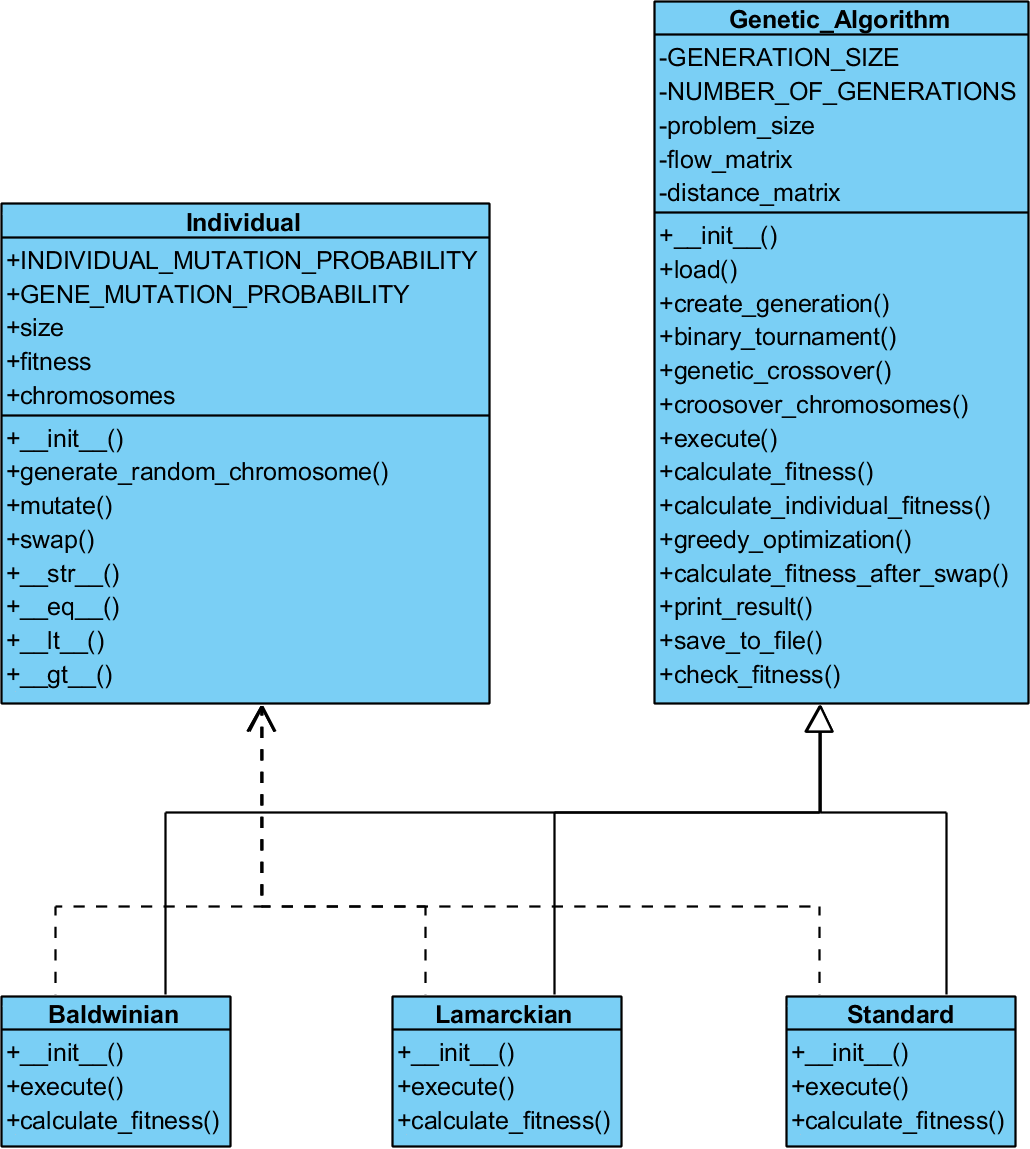
\includegraphics[width=1\textwidth]{../images/class-diagram}
  \caption{Diagrama de clases del proyecto}
  \label{fig:class-diagram}
\end{figure}

\newpage

Como \textbf{operador de cruce} se ha utilizado \textbf{recombinación en un punto}. Esta técnica permite cortar a ambos padres en un punto y recombinar sus trozos. La imagen \ref{fig:recombinacion-por-punto} representa este algoritmo, aunque específicamente en este problema hay que tener cuidado de no repetir sus cromosomas, pasando al siguiente número en caso de que ya exista.

\begin{figure}[H]
  \centering
  \captionsetup{justification=centering}
  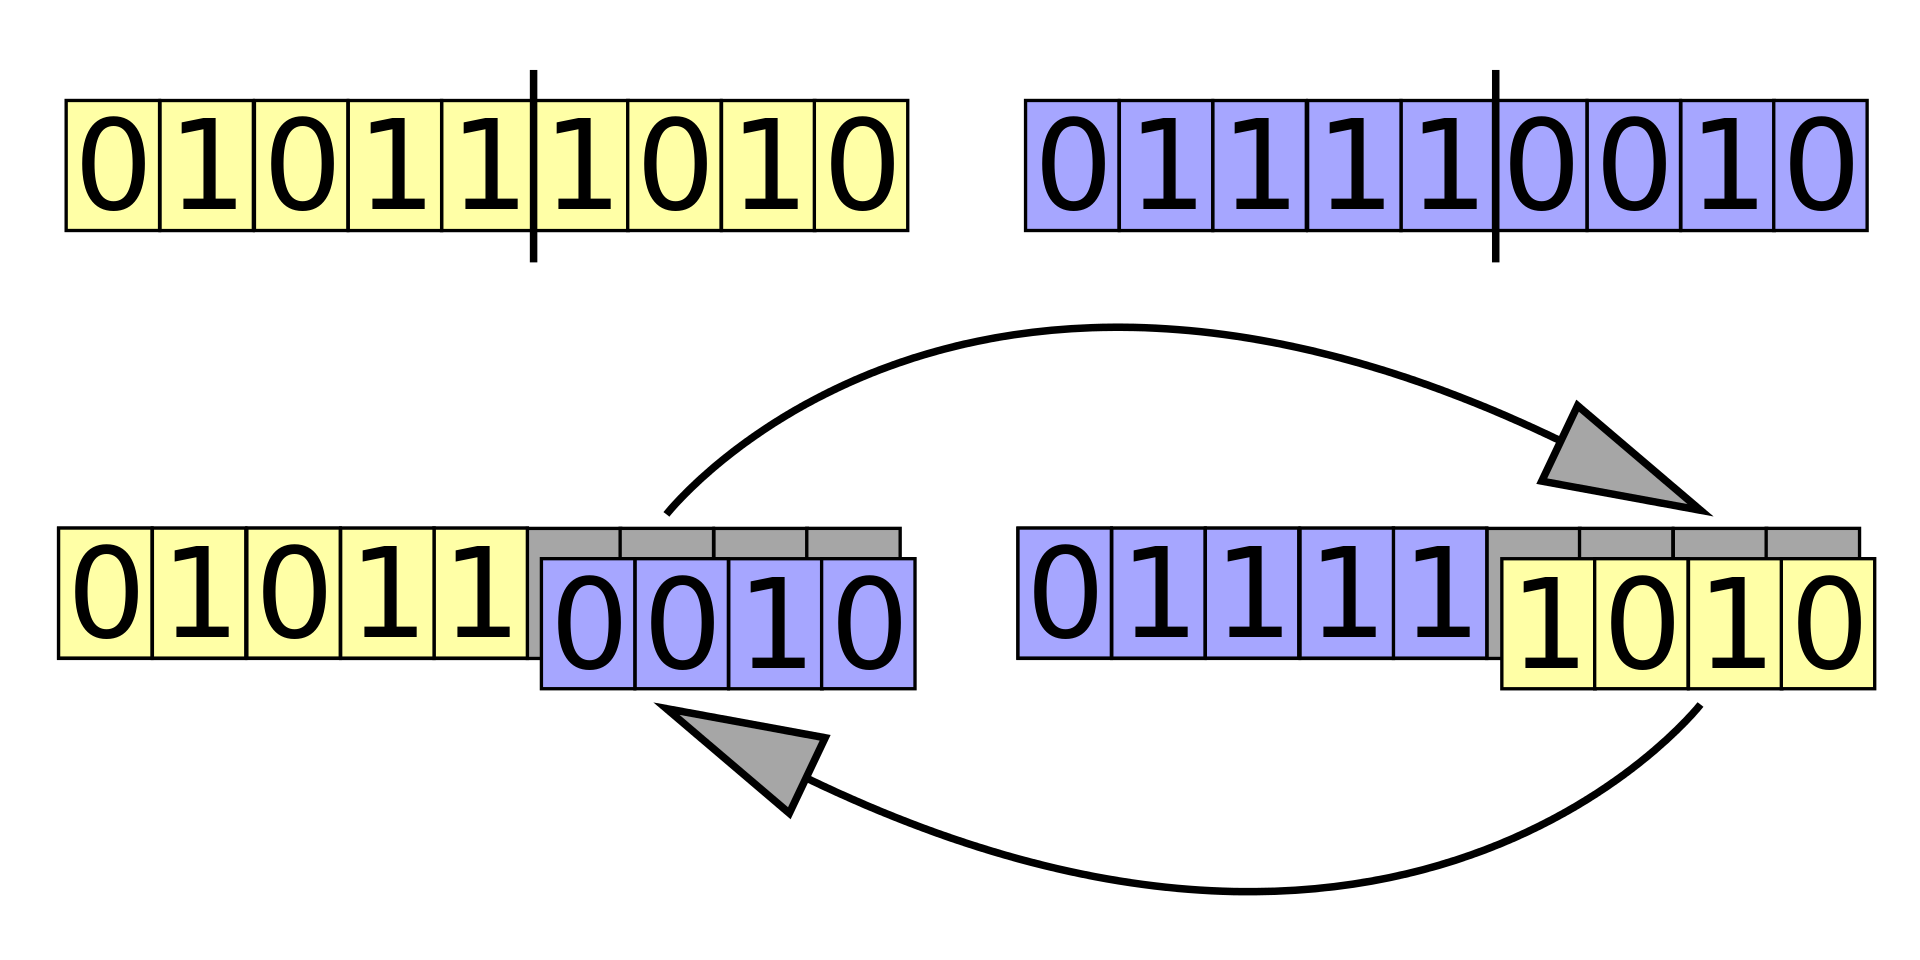
\includegraphics[width=0.5\textwidth]{../images/recombinacion-por-punto}
  \caption{Representación gráfica de la recombinación por punto}
  \small Referencia: Wikipedia.
  \label{fig:recombinacion-por-punto}
\end{figure}

Los tres algoritmos comparten la ejecución básica, ya que solo se diferencian en la manera de calcular el fitness de los individuos. En el listado \ref{lst:base-execution} puede verse el pseudocódigo de esta ejecución común.

\begin{lstlisting}[caption={Ejecución base de los algoritmos}, label={lst:base-execution}]
leer_fichero()
generacion_actual = crear_generacion()
generacion_actual.calcular_fitness()

for i=0..NUM_GENERACIONES:
    for j=0..TAM_GENERACION:
        padre1 = torneo_binario(generacion_actual)
        padre2 = torneo_binario(generacion_actual) && padre1 != padre2
        
        hijo1, hijo2 = recombinar(padre1, padre2)
        hijo1.mutar()
        hijo2.mutar()
        
        nueva_generacion.añadir(hijo1, hijo2)
        
    mejor = generacion_actual.obtener_mejor()
    nueva_generacion.sustituior_peor_por(mejor)
    generacion_actual = nueva_generacion
    generacion_actual.calcular_fitness()

    comprobar_que_el_mejor_no_se_repite_o_reinicializar(mejor)

return generacion_actual.obtener_mejor()
\end{lstlisting}

En la linea 21, la única no explicada anteriormente, se comprueba que el mejor individuo de la población no lleva repitiéndose más veces que las permitidas, y de ser así reinicia la población conservando el mejor individuo de la anterior.

\section{Algoritmo estándar}

De las tres implementaciones de la que consta la práctica, el algoritmo estándar fue el primero que se programó. Su fitness es el más sencillo, ya que basta con aplicar la fórmula \ref{formula:sum} explicada en la introducción.

\section{Variantes evolutivas}

La técnica de optimización local aplicada es un algoritmo \textit{greedy 2-opt}. El fragmento de pseudocódigo \ref{lst:greedy-2opt} muestra cómo funciona.

\begin{lstlisting}[caption={Optimización greedy 2-opt}, label={lst:greedy-2opt}]
S = candidato inicial con coste c(S) 
mejor = S
for i=1..n:
    for j=i+1..n:
        T = S tras intercambiar i con j 
        if c(T) < c(S):
            S=T
return S
\end{lstlisting}

Se ha simplificado con respecto a la versión propuesta en el guión de prácticas eliminando el bucle \texttt{while}, ya que es prácticamente imposible que tras iterar cuadráticamente sobre el tamaño del problema \texttt{S} y \texttt{T} terminen siendo iguales, y tras realizar pruebas se comprobó que esto nunca sucede, por lo que se decidió eliminar de la implementación.

Por otro lado Python, por ser un lenguaje interpretado, funciona especialmente lento en comparación a otros lenguajes compilados, por lo que se ha dedicado un esfuerzo extra en intentar optimizar todo lo posible el algoritmo. Concretamente, y como fue propuesto en clase por el profesor Berzal, se ha diseñado una función específica para recalcular el fitness de los individuos tras intercambiar sus cromosomas (línea 5 del listado \ref{lst:greedy-2opt}), modificando solo los valores que han cambiado. Así, se ha conseguido reducir la complejidad de esa función en concreto de $O(n^2)$ a $O(n)$. 

\subsection{Variante lamarckiana}

Esta variante está basada en la teoría evolutiva del naturalista francés \textbf{Jean-Baptiste Lamarck} (1744-1829), quien afirmaba que las mejoras fisiológicas que obtenía un individuo a lo largo de su vida  quedaban grabadas en sus genes, por lo que sus descendientes adquirían esta mejoras en su código genético.

Así, tras obtener un individuo optimizado con la función presentada en el litado \ref{lst:greedy-2opt}, el individuo original el sustituido por su versión mejorada.

\subsection{Variante baldwiniana}

Esta variante está basada en la teoría evolutiva del psicólogo estadounidense \textbf{James Mark Baldwin} (1861-1934), quien afirmaba que las mejoras fisiológicas de un individuo obtenidas a lo largo de su vida no se graban en sus genes, por lo que su descendencia no las obtiene.

Así, tras aplicar una optimización local en cada generación, éstas no se usan para generar la siguiente población, sino que \textit{mueren} con sus individuos.
\chapter{Resultados}
\label{chap:res}

Tras implementar y ejecutar las tres variantes del algoritmo genético se pasó a analizar los resultados.

Para los resultados presentados en esta sección se han usado los siguientes parámetros.

En lo que respecta a la población,

\begin{itemize}
	\item \textbf{Tamaño de población.} 60
	\item \textbf{Número de generaciones.} 100
	\item \textbf{Máximo número de repeticiones del mejor individuo.} 20
\end{itemize}

Inicialmente se probó con tamaños de población más pequeños y mayor número de generaciones, pero el hecho de tener pocos individuos hacía que se obtuviera rápidamente el mínimo de la ejecución, y por lo general no solían ser muy buenos.

Por otro lado, la variable \texttt{Máximo número de repeticiones del mejor individuo} indica cuántas veces puede repetirse el mejor individuo una generación tras otra antes de reinicializar la población, asumiendo que ese individuo es especialmente bueno y la población actual no va a mejorarlo.

En lo que respecta a los individuos,

\begin{itemize}
	\item \textbf{Probabilidad individual de mutación.} 50\%
	\item \textbf{Probabilidad de mutación de cada cromosoma.} 5\%
\end{itemize}

Se ha intentado no depender mucho en el RNG\footnote{Random Number Generation} para obtener los resultados, por lo que las probabilidades de mutación no son muy altas.

\section{Comparación de resultados}

En el gráfico \ref{fig:comparacion-3} se presentan los resultados tras ejecutar los tres algoritmos. En el anexo \ref{anexo:results} pueden verse tanto el tiempo de ejecución como el fitness y los cromosomas del mejor individuo de cada ejecución.

\begin{figure}[H]
  \centering
  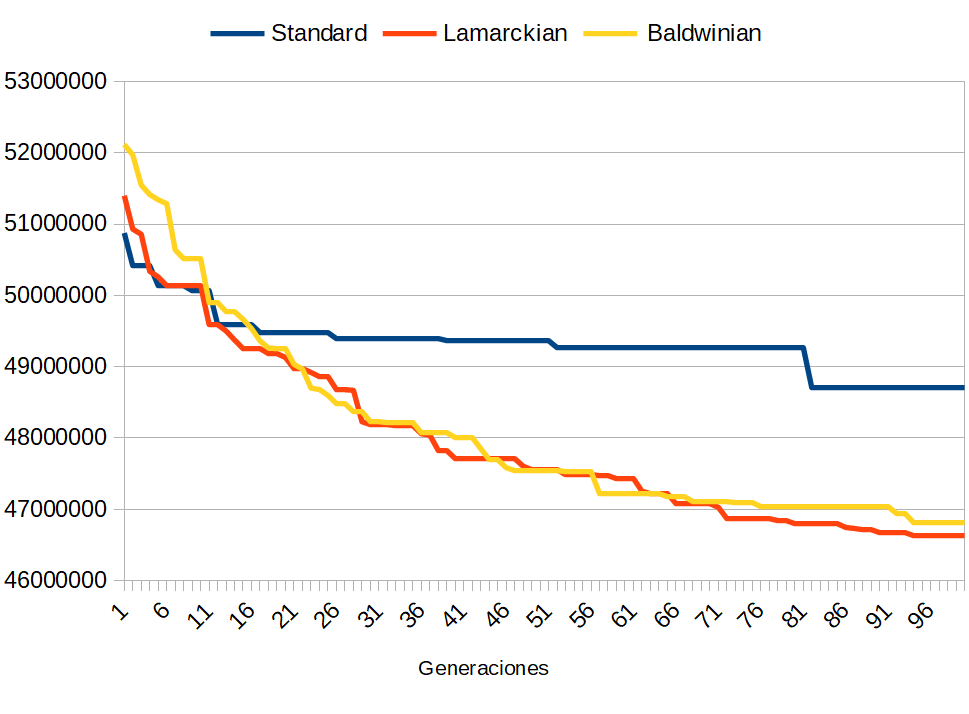
\includegraphics[width=1\textwidth]{../images/comparacion-3}
  \caption{Comparación del resultado de la ejecución de los tres algoritmos}
  \label{fig:comparacion-3}
\end{figure}

Se han repetido las ejecuciones varias veces con resultados muy parecidos, por lo que se concluye que estos datos son representativos.

Como puede verse, el algoritmo que peor desempeño tiene es el estándar, ya que mejora muy poco y muy lentamente a lo largo de su ejecución. Por otro lado, sus dos variantes tienen resultados bastante parecidos, aunque la implementación lamarckiana da mejores resultados. Esto tiene sentido, ya que transmitir las mejoras de un individuo en sus cromosomas, aunque no sea realista, proporciona mejores resultados que de no hacerlo.


\section{Mejor resultado obtenido}

Actualmente, el mejor resultado obtenido ha sido con la ejecución de la implementación \textbf{lamarckiana} con un fitness de \textbf{46634000}, un $\sim$1.06\% mayor que la cota inferior global conocida (44095032). Sus cromosomas pueden verse en el anexo \ref{anexo:best}.
\chapter{Conclusiones}
\label{chap:concl}

Los algoritmos genéticos son muy profundos y, aunque esta práctica me ha servido sólo como introducción, me alegro mucho de haberla realizado. 

Además, el hecho de haber utilizado un lenguaje interpretado, más lento, me ha llevado a tener que optimizar la práctica, algo que de haber obtenido unos tiempos de ejecución razonablemente bajos no me habría planteado hacer.

La mayoría de mis compañeros ya tenían nociones básicas y conocían los conceptos de los algoritmos genéticos por haberlos visto en el Grado, pero en la UCLM no se estudian así que yo apenas sí los conocía de oídas. Por eso, aunque me haya podido costar algo más de trabajo realizar la práctica, creo que me ha resultado especialmente útil.


% \input{chapters/06_Referencias}
\chapter{Anexos}
\label{chap:anexos}

\section{Anexo 1. Resultados de la comparación de los tres algoritmos}
\label{anexo:results}

\subsection*{Standard}

\begin{itemize}
	\item \textbf{Tiempo de ejecución.} $\sim$178 segundos
	\item \textbf{Fitness del mejor elemento.} 48711852
	\item \textbf{Cromosomas} [173, 175, 7, 223, 0, 128, 94, 96, 242, 31, 167, 18, 42, 108, 250, 163, 69, 116, 9, 237, 62, 95, 55, 151, 192, 48, 155, 232, 138, 122, 22, 114, 153, 50, 60, 57, 35, 51, 113, 177, 189, 49, 75, 239, 84, 93, 101, 201, 188, 156, 91, 214, 159, 193, 70, 176, 222, 152, 241, 213, 37, 81, 40, 29, 210, 245, 72, 102, 120, 164, 126, 211, 149, 33, 104, 244, 89, 76, 230, 165, 252, 179, 131, 87, 234, 199, 197, 202, 220, 145, 28, 140, 187, 54, 132, 63, 23, 61, 219, 3, 27, 161, 228, 56, 107, 243, 154, 215, 125, 59, 246, 181, 224, 67, 196, 162, 180, 111, 77, 19, 52, 226, 12, 68, 58, 249, 65, 8, 235, 254, 182, 227, 115, 73, 168, 236, 143, 88, 218, 5, 4, 16, 11, 10, 166, 47, 147, 169, 71, 26, 233, 109, 41, 205, 79, 53, 231, 20, 160, 99, 203, 32, 198, 80, 36, 44, 141, 146, 38, 30, 103, 85, 216, 119, 129, 112, 92, 206, 78, 100, 121, 134, 13, 190, 221, 209, 2, 217, 139, 124, 191, 25, 90, 238, 15, 106, 135, 186, 117, 158, 212, 98, 45, 118, 184, 46, 24, 21, 64, 127, 14, 74, 66, 130, 157, 110, 253, 150, 133, 225, 82, 248, 172, 97, 1, 123, 170, 142, 105, 144, 247, 200, 148, 86, 183, 229, 194, 39, 17, 174, 34, 251, 137, 43, 136, 207, 204, 240, 255, 208, 185, 178, 83, 195, 6, 171]
\end{itemize}

\subsection*{Lamarckian}
\label{anexo:best}

\begin{itemize}
	\item \textbf{Tiempo de ejecución.} $\sim$7552 segundos
	\item \textbf{Fitness del mejor elemento.} 46634000
	\item \textbf{Cromosomas} [169, 56, 148, 224, 235, 32, 12, 250, 103, 243, 50, 65, 150, 192, 60, 254, 214, 147, 255, 173, 95, 241, 76, 45, 137, 26, 191, 167, 126, 84, 248, 125, 101, 201, 186, 58, 245, 199, 88, 4, 17, 228, 107, 178, 0, 180, 197, 226, 23, 31, 53, 156, 110, 62, 217, 68, 105, 122, 203, 188, 206, 81, 161, 189, 253, 54, 159, 165, 129, 93, 231, 51, 18, 43, 130, 135, 212, 116, 154, 72, 112, 86, 21, 160, 221, 9, 90, 118, 98, 79, 184, 193, 213, 215, 5, 89, 66, 113, 70, 82, 151, 67, 171, 209, 97, 227, 195, 142, 102, 205, 20, 219, 111, 61, 237, 96, 52, 49, 174, 7, 211, 37, 69, 64, 104, 223, 55, 15, 200, 41, 247, 157, 119, 74, 39, 35, 181, 216, 220, 128, 27, 6, 106, 11, 34, 141, 179, 83, 131, 204, 230, 194, 40, 145, 138, 46, 77, 59, 10, 28, 225, 244, 120, 187, 190, 149, 71, 196, 42, 123, 182, 47, 172, 152, 121, 124, 198, 36, 94, 78, 164, 99, 146, 218, 24, 87, 117, 13, 44, 249, 108, 14, 239, 242, 234, 33, 85, 163, 1, 238, 75, 8, 251, 38, 166, 229, 185, 127, 240, 162, 202, 3, 233, 246, 144, 73, 236, 133, 153, 57, 30, 155, 177, 115, 140, 222, 183, 109, 100, 176, 19, 16, 232, 158, 168, 207, 134, 63, 208, 136, 29, 132, 170, 252, 92, 91, 48, 2, 210, 143, 175, 114, 80, 139, 22, 25]
\end{itemize}


\subsection*{Baldwinian}

\begin{itemize}
	\item \textbf{Tiempo de ejecución.} $\sim$7029 segundos
	\item \textbf{Fitness del mejor elemento.} 46815666
	\item \textbf{Cromosomas} [20, 50, 153, 186, 85, 96, 162, 53, 201, 250, 70, 221, 74, 194, 214, 0, 103, 145, 19, 12, 197, 160, 152, 248, 172, 158, 150, 232, 14, 97, 2, 33, 92, 78, 218, 130, 42, 121, 180, 45, 135, 244, 211, 63, 168, 31, 139, 5, 89, 165, 247, 192, 148, 39, 183, 190, 25, 251, 65, 226, 163, 100, 128, 188, 159, 56, 255, 44, 208, 38, 125, 67, 126, 93, 241, 131, 230, 87, 199, 237, 27, 95, 206, 52, 82, 59, 252, 141, 203, 117, 107, 24, 13, 134, 127, 3, 90, 32, 105, 220, 98, 176, 88, 200, 146, 124, 102, 187, 84, 8, 73, 253, 240, 51, 182, 207, 222, 104, 149, 119, 198, 108, 181, 242, 75, 238, 204, 22, 16, 216, 157, 254, 154, 151, 166, 129, 58, 114, 174, 120, 116, 35, 26, 169, 6, 202, 17, 106, 28, 227, 76, 109, 137, 179, 10, 72, 40, 205, 1, 60, 210, 15, 225, 41, 57, 43, 47, 223, 55, 101, 49, 142, 178, 23, 193, 115, 91, 122, 118, 235, 184, 140, 189, 94, 86, 156, 246, 138, 99, 213, 245, 136, 212, 224, 219, 234, 144, 164, 34, 71, 233, 29, 175, 54, 239, 249, 143, 48, 36, 209, 9, 30, 133, 111, 11, 66, 110, 37, 217, 62, 147, 64, 177, 228, 21, 77, 161, 167, 191, 196, 68, 18, 69, 112, 229, 46, 123, 79, 83, 80, 231, 81, 4, 173, 185, 113, 236, 170, 215, 61, 195, 7, 155, 171, 132, 243]

\end{itemize}

\newpage

\section{Anexo 2. Código fuente de la práctica}
\label{anexo:code}

\subsection*{main.py}

\begin{lstlisting}[language=python]
from auxiliary import *

from standard import Standard
from baldwinian import Baldwinian
from lamarckian import Lamarckian


standard   = Standard()
baldwinian = Baldwinian()
lamarckian = Lamarckian()


if __name__ == '__main__':

    elapsed_time = execute_algorithm( standard, 'tai256c.dat' )
    print("Standard executing time: {:.3f}s\n".format(elapsed_time))

    elapsed_time = execute_algorithm( baldwinian, 'tai256c.dat' )
    print("Baldwinian executing time: {:.3f}s\n".format(elapsed_time))

    elapsed_time = execute_algorithm( lamarckian, 'tai256c.dat' )
    print("Lamarckian executing time: {:.3f}s\n".format(elapsed_time))
\end{lstlisting}

\newpage

\subsection*{auxiliary.py}
\begin{lstlisting}[language=python]
import os
import time

from genetic_algorithm import GeneticAlgorithm
from standard import Standard

DATA_DIR = os.path.join('src', 'data', 'qap')


def get_data_files( dir ):
    """
    Reference https://stackoverflow.com/questions/3207219/how-do-i-list-all-files-of-a-directory
    """
    def exists(file):
        return os.path.isfile(os.path.join(dir, file))

    return [file for file in os.listdir(dir) if exists(file)]


def execute_algorithm( algorithm, datafile ):
    """
    Executes a genetic algorithm and returns its computing time
    """
    if issubclass(type(algorithm), GeneticAlgorithm):
        start_time = time.time()
        algorithm.execute( datafile )
        return time.time() - start_time

    else:
        raise Exception('The algorithm is not a subclass of GeneticAlgorithm')


def check_files( ):
    """
    Runs the Standar genetic algorithm with all the files and checks for AssertionErrors, that happens when the files are not well-structured Corret structure: Problem size, flow matrix and distance matrix with size equal to the problem size
    Current erros: 19
    """
    n_assertion_err = 0
    for file in get_data_files( DATA_DIR ):
        try:
            execute_algorithm( Standard(), file )
        except AssertionError:
            print("=========== AssertionError exception on file", file)
            n_assertion_err += 1
    print(n_assertion_err)

\end{lstlisting}

\subsection*{genetic\_algorithm.py}
\begin{lstlisting}[language=python]
"""
Parent class of the rest of the algorithms holding its variables
"""

import os
import sys
import random
from copy import deepcopy

from individual import Individual


class GeneticAlgorithm:
    """
    Parent class of the rest of algorithms, holding their common functions and variables
    """

    def __init__(self):
        """
        Fixed variables
        """
        self.GENERATION_SIZE       = 60
        self.NUMBER_OF_GENERATIONS = 100
        self.MAX_NUMBER_REPETITION_BEST_ONE = 20
        """
        Problem variables
        """
        self.problem_size    = -1
        self.flow_matrix     = []
        self.distance_matrix = []

        """
        Counts the number of times the best individual of a generation is repeated to reinitialise it
        """
        self.last_best_one = Individual(0)
        self.repetition_best_one = 0

        """
        Stores the best one of each generation to (manually) make a graph
        """
        self.bests = []
        

    def load(self, filename):
        """
        Parses a file and stores its flow and distance matrices as class variables that can be accessed by the class inheriting from it
        """
        self.filename = filename
        datafile = os.path.join('src', 'data', 'qap', self.filename)

        if os.path.isfile( datafile ):
            with open( datafile, 'r' ) as f:
                lines = f.readlines()
                lines = [line.split() for line in lines]
                lines = [list(map(int, line)) for line in lines if line != []] # avoids empty lines

                self.problem_size = int(lines[0][0])

                assert(len(lines) == self.problem_size*2+1) # checks the file has a correct structure

                self.flow_matrix = lines[1:self.problem_size+1]
                self.distance_matrix = lines[self.problem_size+1:]

        else:
            raise FileNotFoundError("Cannot find file {}".format( datafile ))


    def create_generation(self):
        """
        Creates a generation with the size of the problem initialised with random individuals
        """
        generation = []
        for i in range(self.GENERATION_SIZE):
            generation.append( Individual( self.problem_size ) )

        return generation


    def binary_tournament(self):
        """
        Randomly selects two different individuals from the current generation and returns the optimal one
        """
        rand_numb1, rand_numb2 = random.sample(range(0, self.GENERATION_SIZE), 2)

        individ1 = self.current_generation[rand_numb1]
        individ2 = self.current_generation[rand_numb2]

        return min([individ1, individ2])


    def genetic_crossover(self, parent1, parent2):
        """
        Mixes the two parent individuals into two children slicing them by a random index and avoiding repeating chromosomes in each child
        """
        slice_index = random.randint(1, self.problem_size-1)

        child1_chrom = self.croosover_chromosomes(slice_index,
                                                  parent1.chromosomes,
                                                  parent2.chromosomes)
        child2_chrom = self.croosover_chromosomes(slice_index,
                                                  parent2.chromosomes,
                                                  parent1.chromosomes)

        assert(len(child1_chrom) == len(child2_chrom) == self.problem_size)

        child1 = Individual( self.problem_size )
        child1.chromosomes = child1_chrom

        child2 = Individual( self.problem_size )
        child2.chromosomes = child2_chrom

        return child1, child2


    def croosover_chromosomes(self, slice_index, parent1, parent2):
        numbers_left = self.problem_size - slice_index
        child = parent1[:slice_index]

        index = slice_index
        while len(child) < self.problem_size:
            if parent2[index] not in child:
                child.append(parent2[index])

            index += 1
            if index >= self.problem_size:
                index = 0

        return child


    def execute(self, datafile):
        """
        Genetic algorithm's execution function. It is inherited by all its children, which will overload the default 'calculate_fitness' function.
        """
        print("Executing algorithm with file {}".format(datafile))

        self.load( datafile )

        self.current_generation = self.create_generation()
        self.calculate_fitness( self.current_generation )

        for i in range( self.NUMBER_OF_GENERATIONS ):
            print("Executing generation {}/{}... Best {}".format(i+1, self.NUMBER_OF_GENERATIONS, self.last_best_one.fitness), end="\r")

            new_generation = []
            for j in range( 0, int(self.GENERATION_SIZE), 2 ): # step = 2
                parent1 = self.binary_tournament()

                parent2 = None
                while parent1 != parent2:
                    parent2 = self.binary_tournament()

                child1, child2 = self.genetic_crossover(parent1, parent2)

                child1.mutate()
                child2.mutate()

                new_generation.append( child1 )
                new_generation.append( child2 )


            """
            Pops out the worst one of the current generation and inserts in its place the best one of the previous generation
            """
            old_best = min( self.current_generation )
            new_worst = max( new_generation )
            new_worst_index = new_generation.index( new_worst )
            new_generation.pop( new_worst_index )
            new_generation.append( old_best )
            self.current_generation = new_generation

            self.calculate_fitness( self.current_generation )

            """
            Check the best one is not stuck being repeated over generations. Otherwise, reinitialise the population keeping the best one
            """
            best_one = min( self.current_generation )
            self.check_best_one_from_generation( best_one )

            self.bests.append(best_one)

        best_one = min( self.current_generation )
        return best_one


    def calculate_fitness(self, generation):
        """
        All the child classes inheriting from this one shall override this function.
        """
        raise NotImplementedError


    def calculate_individual_fitness(self, individual):
        """
        Calculates the fitness of a single individual and checks that it is not greater than the possible maximum.
        """
        new_fitness = 0
        for i in range(self.problem_size):
            for j in range(self.problem_size):
                chrom_i = individual.chromosomes[i]
                chrom_j = individual.chromosomes[j]

                new_fitness += self.flow_matrix[i][j] * \
                               self.distance_matrix[chrom_i][chrom_j]

        self.check_fitness( new_fitness )
        return new_fitness


    def greedy_optimization(self, individual):
        """
        Greedy 2-opt algorithm implementing the pseudocode given on the problem statement. The do/while loop has been ommited from the algorithm as it is virtually impossible that after all the permutations S == best, and even though if that was the case it would not change for executing for loops again.
        """
        S = deepcopy( individual )
        S.fitness = self.calculate_individual_fitness( S )

        best = deepcopy( S )

        for i in range( S.size ):
            for j in range(i + 1, S.size):
                T = deepcopy( S )
                T.chromosomes[i] = S.chromosomes[j]
                T.chromosomes[j] = S.chromosomes[i]

                self.calculate_fitness_after_swap( S, T, i, j )

                if T < S:
                    S = deepcopy( T )

        return S


    def calculate_fitness_after_swap(self, S, T, i, j):
        """
        Instead of calculating again the whole fitness, it is only a matter of calculing the chromosomes that have been changed, reducing complexity from n^2 to 2n
        """
        new_fitness = T.fitness
        chrom_S_i = S.chromosomes[i]
        chrom_S_j = S.chromosomes[j]
        chrom_T_i = T.chromosomes[i]
        chrom_T_j = T.chromosomes[j]

        for k in range(self.problem_size):
            chrom_S_k = S.chromosomes[k]
            chrom_T_k = T.chromosomes[k]

            # recalculate i
            new_fitness -= self.flow_matrix[i][k] * \
                           self.distance_matrix[chrom_S_i][chrom_S_k]

            new_fitness -= self.flow_matrix[i][k] * \
                           self.distance_matrix[chrom_T_i][chrom_T_k]

            # recalculate j
            new_fitness -= self.flow_matrix[j][k] * \
                           self.distance_matrix[chrom_S_j][chrom_S_k]

            new_fitness += self.flow_matrix[j][k] * \
                           self.distance_matrix[chrom_T_j][chrom_T_k]

            # recalculate the rest of the values of the loop
            if k not in [i, j]:
                # recalculate i
                new_fitness -= self.flow_matrix[k][i] * \
                               self.distance_matrix[chrom_S_k][chrom_S_i]

                new_fitness += self.flow_matrix[k][i] * \
                               self.distance_matrix[chrom_T_k][chrom_T_i]

                # recalculate j
                new_fitness -= self.flow_matrix[k][j] * \
                               self.distance_matrix[chrom_S_k][chrom_S_j]

                new_fitness += self.flow_matrix[k][j] * \
                               self.distance_matrix[chrom_T_k][chrom_T_j]


    def check_best_one_from_generation(self, best_one):
        """
        Check the best one is not stuck being repeated over generations. Otherwise, reinitialise the population keeping the best one
        """
        if best_one == self.last_best_one:
            self.repetition_best_one += 1
            if self.repetition_best_one > self.MAX_NUMBER_REPETITION_BEST_ONE:
                print("\nStuck population! Best one {}. Reinitialising...".format(best_one.fitness))
                self.reinitialise_population( best_one )
                self.repetition_best_one = 0

        else:
            self.repetition_best_one = 0

        self.last_best_one = best_one


    def reinitialise_population(self, best_one):
        """
        Generates another random generation, pops one individual at random and inserts the best one from the previous generation
        """
        self.current_generation = self.create_generation()
        self.calculate_fitness( self.current_generation )
        self.current_generation.pop()
        self.current_generation.append(best_one)


    def print_result(self, best_one):
        """
        Prints the final result.
        """
        print("________________________________________________")
        print("Recombination operator: Crossover")
        print("Mutation operator: Index swap")
        print("Problem size: ", self.problem_size)
        print("Number of generations: ", self.NUMBER_OF_GENERATIONS)
        print("Generation size: ", self.GENERATION_SIZE)
        print("Fitness of the final best individual: ", best_one.fitness)
        print("Chromosomes:\n", best_one.chromosomes )


    def save_to_file(self, best_one):
        """
        Redirects the stdout to a file and saves the results
        """
        filename = 'result.txt'
        filename = os.path.join('results', filename)
        f = open( filename, 'w')

        orig_stdout = sys.stdout
        sys.stdout = f

        self.print_result( best_one )

        sys.stdout = orig_stdout
        f.close()


    def check_fitness(self, fitness):
        """
        Check the fitness is not lesser than the possible value
        """
        if self.filename == 'tai256c.dat' and fitness < 44095032:
            raise Exception("Fitness cannot be lesser than 44095032 on file \
                             tai256c, current ", fitness)

\end{lstlisting}

\newpage

\subsection*{standard.py}
\begin{lstlisting}[language=python]

from genetic_algorithm import GeneticAlgorithm
from individual import Individual

class Standard(GeneticAlgorithm):
    """
    Standard implementation of the genetic algorithm
    """

    def __init__(self):
        super(Standard, self).__init__()


    def execute(self, datafile):
        """
        Loads the data, creates the first generation and executes the genetic algorithm on each generation overloading and executing the child 'calculate_fitness' function. Finally returns the best of 'em all.
        """
        best_one = super().execute( datafile )
        super().print_result( best_one )
        super().save_to_file( best_one )

        return best_one


    def calculate_fitness(self, generation):
        """
        Calculate the fitness of each individual on the generation
        """
        for individual in generation:
            individual.fitness = super().calculate_individual_fitness(individual)
\end{lstlisting}

\newpage

\subsection*{lamarckian.py}
\begin{lstlisting}[language=python]
from genetic_algorithm import GeneticAlgorithm
from individual import Individual


class Lamarckian(GeneticAlgorithm):
    """
    Lamarckian implementation of the genetic algorithm
    """

    def __init__(self):
        super(Lamarckian, self).__init__()


    def execute(self, datafile):
        """
        Loads the data, creates the first generation and executes the genetic algorithm on each generation overloading and executing the child 'calculate_fitness' function. Finally returns the best of 'em all.
        """
        best_one = super().execute( datafile )
        super().print_result( best_one )
        super().save_to_file( best_one )
        return best_one


    def calculate_fitness(self, generation):
        """
        Optimizes the individual and saves the changes for them to be inherited
        by its offspring so next generation have it. Works in the say proposed
        by the biologist J. B. Lamark.
        """
        for individual in generation:
            individual = super().greedy_optimization( individual )
\end{lstlisting}

\newpage

\subsection*{baldwinian.py}
\begin{lstlisting}[language=python]
from genetic_algorithm import GeneticAlgorithm
from individual import Individual


class Baldwinian(GeneticAlgorithm):
    """
    Baldwinian implementation of the genetic algorithm
    """

    def __init__(self):
        super(Baldwinian, self).__init__()


    def execute(self, datafile):
        """
        Loads the data, creates the first generation and executes the genetic algorithm on each generation overloading and executing the child 'calculate_fitness' function. Finally returns the best of 'em all.
        """
        best_one = super().execute( datafile )
        super().print_result( best_one )
        super().save_to_file( best_one )
        return best_one


    def calculate_fitness(self, generation):
        """
        Optimizes the individual but only changes its fitness without letting the optimisation, thus not allowing the optimization to be in it offspring. Works in the way propposed by the psicologist J. M. Baldwin.
        """
        for individual in generation:
            optimized_individual = super().greedy_optimization( individual )
            individual.fitness = optimized_individual.fitness
\end{lstlisting}

\newpage

\subsection*{individual.py}
\begin{lstlisting}[language=python]
import math
import random


class Individual:

    def __init__(self, size):
        self.INDIVIDUAL_MUTATION_PROBABILITY = 0.5
        self.GENE_MUTATION_PROBABILITY       = 0.05

        self.size    = size
        self.fitness = math.inf
        self.generate_random_chromosome( size )


    def generate_random_chromosome(self, size):
        self.chromosomes = list(range(size))
        random.shuffle(self.chromosomes)


    def mutate(self):
        if self.INDIVIDUAL_MUTATION_PROBABILITY > random.random():
            for chromosome in self.chromosomes:
                if self.GENE_MUTATION_PROBABILITY > random.random():
                    index1, index2 = random.sample(range(0, self.size), 2)
                    self.swap( index1, index2 )


    def swap(self, index1, index2):
        val1 = self.chromosomes[index1]
        val2 = self.chromosomes[index2]
        self.chromosomes[index1] = val2
        self.chromosomes[index2] = val1


    def __str__(self):
        return str(self.chromosomes)


    def __eq__(self, other):
        if not isinstance(other, Individual):
            return False

        equal_size = self.size == other.size
        equal_chrom = set(self.chromosomes) == set(other.chromosomes)

        return equal_size and equal_chrom


    def __lt__(self, other):
        if not isinstance(other, Individual):
            return False

        return self.fitness < other.fitness


    def __gt__(self, other):
        if not isinstance(other, Individual):
            return False

        return self.fitness > other.fitness
\end{lstlisting}

\newpage \
\thispagestyle{empty}
\end{document}
